%=======================================================
\section{Use Case Analysis}
%=======================================================

%=======================================================
\section{\acl{DTE} Proposal}
%=======================================================

%=======================================================
\section{Implemented Solution}
%=======================================================

\subsection{The Trauma Management Use Case}

The healthcare sector is characterized by heterogeneity (see \Cref{ssec:dimensions}) and data integration challenges due to the presence of legacy systems and rich data that often lack adherence to shared standards.
These aspects, united with the need to track complex operations in real-time to enhance coordination among medical teams and improve the patient's journey~\cite{croatti2020jms,ricci2022dthealthcare}, make healthcare use cases perfect candidates for \ac{DT} ecosystems~\cite{10178878}.

Major Trauma Management, originally described in \cite{ricci2022wodt}, involves the coordination of rescue missions to track patient conditions from the initial contact of the medical team over the whole journey in the emergency department.

Typically, when \ac{CEU} operators receive an emergency call, they collect initial information and initiates a new \emph{mission} for each victim of the trauma.
An \emph{ambulance} and a designated \emph{rescuer} are then dispatched to reach the patient, provide first aid and eventually lead them to the hospital.
%
Upon arrival at the trauma location, the rescue crew establishes contact with the \emph{patient}, who may be identified via their health insurance card.
Depending on the patient's condition, a destination trauma center is selected and, during the journey, the patient is continuously monitored.

The trauma management process requires coordination across multiple departments, each relying on diverse systems, which we (safely) assume for the scope of our use case to be developed using different technologies due to the fragmented evolution of electronic health systems.

Specifically, we assume to have two main subsystems: emergency call management, which includes mission planning, and pre-hospital patient monitoring.
%
We further assume these systems to be already \ac{DT} enabled, but using different technologies, namely \ac{WLDT} for the emergency call management, \azureTwin{} for patient monitoring and Eclipse Ditto for the national registry of healthcare users.
%
Figure \ref{fig:use-case-diagram} depicts a possible \ac{HWoDT}-based \ac{DTE} implementation joining \acp{DT} of different systems in a coherent view.
%
The use case implementation and the complete description of the use case processes are available on GitHub\footnote{\url{https://github.com/Web-of-Digital-Twins/major-trauma-management-case-study}}.


\begin{figure}[t]
  \centering
  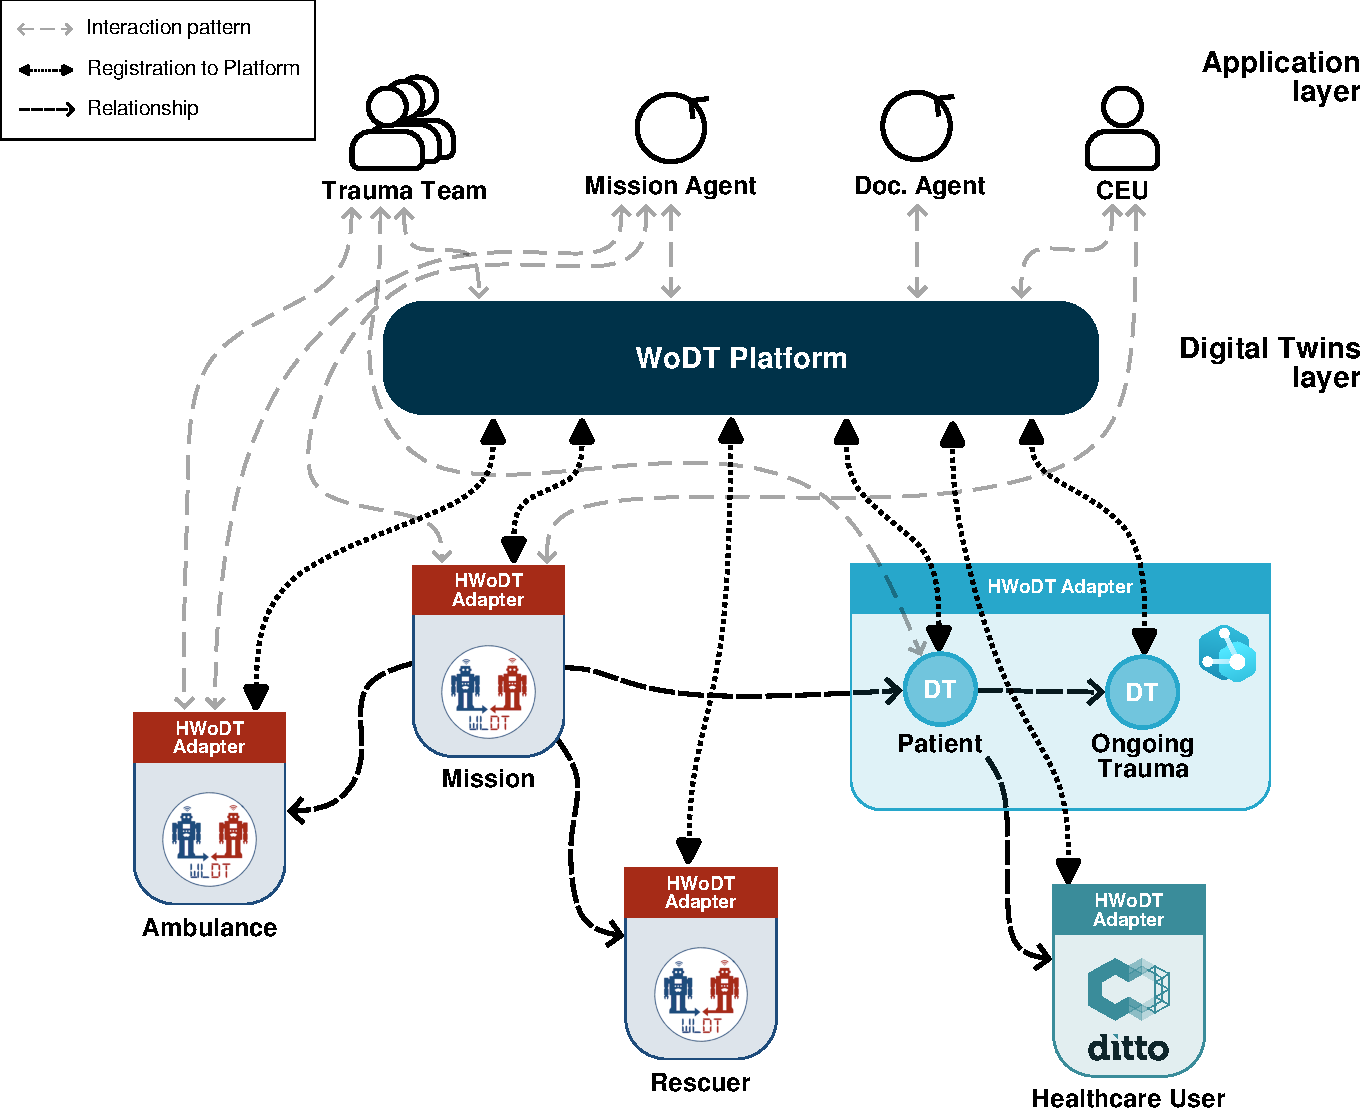
\includegraphics[width=\columnwidth]{figures/hwodt/major-trauma-management.pdf}
  \caption{The \ac{HWoDT}-based \ac{DTE} for the trauma management case study. \acp{DT} implemented with different technologies (WLDT, Ditto, Azure) become interoperable through the HWoDT Adapters and are integrated through the WoDT Platform. 
  Black dotted arrows represent the interaction with the platform, black dashed arrows represent relationships between \acp{DT} while grey arrows represent the interaction between consumers, the platform and \acp{DT}.
  }
  \label{fig:use-case-diagram}
\end{figure}


\subsection{Implementing a \acs{HWoDT} Ecosystem}

The first step towards creating a \ac{HWoDT} \ac{DTE} is to analyze the current state of the system and identify available \acp{DT}, evaluating their modeling capabilities, and understanding the underlying technologies they rely on.
%
Then, the ecosystem model can be refined by introducing relationships between \acp{DT}, derived from domain knowledge, especially where explicit relationships are not supported by the \ac{DT} technology.

The next step is identifying the membership criteria for the ecosystem. These are usually informed by application-specific requirements. 
%
Through the \ac{HWoDT} applications can compose dedicated \acp{DTE} that support their operations, joining only the \acp{DT} they are interested in.
%
In our example, we create one global ecosystem to provide a unified view of ongoing rescue processes.

After this analysis phase, the first step towards implementation is achieved adapting the \acp{DT} to the \ac{HWoDT} uniform interface through \emph{adapters} (\Cref{ssec:adapters}).
\Cref{fig:use-case-diagram} shows the different \acp{DT} each mapped through the relative technology adapter. 
%
Reusing existing adapters is mostly a matter of configuration (e.g., API keys, connection details). 
In this phase, the semantic mapping to build the \ac{DTKG} is the most crucial step. 
For instance, in the example we represent healthcare resources using the HL7 FHIR\footnote{\url{https://www.hl7.org/fhir/}} standard in the \ac{KG}.

At this stage \acp{DT} are already uniformly reachable by consumers, and can be accessed as-a-service.

Deploying the \ac{WoDT} platform and registering \acp{DT} to it further completes the \ac{HWoDT} providing ecosystem-wide services to inspect and monitor the state of the \ac{DTE}.

Finally, applications can now leverage both the individual \acp{DT}' uniform interface and the \ac{WoDT} platform services to implement their business logic.
For instance, the \emph{Mission Agent} (\Cref{fig:use-case-diagram}, top) in the use case can be developed to observe the \ac{DTE} \ac{KG}, react to new missions being created and find free resources to assign with a SPARQL query like the one in \Cref{lst:ambulance-rescuer-query}.

\lstinputlisting[
    label={lst:ambulance-rescuer-query},
    caption={SPARQL Query performed by the Mission Agent to obtain the available ambulances and rescuers with the appropriate qualification.},
]{listings/hwodt/use-case/ambulance-rescuer-query.rq}

\subsection{Benefits and Limitations}
\label{ssec:benefits-limitations}

\note{Maybe move this section somewhere else e.g. conclusion}

The showcase of the implementation and exploitation of an \ac{HWoDT} ecosystem allows us to highlight benefits and discuss limitations of the approach.

\paragraph{Decoupling and Interoperability}
The main benefit is the decoupling from the underlying heterogeneous technologies achieved through the \ac{HWoDT} uniform interface.
%
As a result, ecosystem-aware applications — such as dashboards and automation tools (e.g., the \emph{Mission Agent}) — can be built using standard Web technologies, treating \acp{DT} as Web resources.

\Cref{fig:comparison-custom-vs-hwodt} highlights the difference in interaction with the \ac{DTE} compared to custom, heterogeneous solutions, when querying across multiple \acp{DT}.
%
Without the \ac{HWoDT}, applications must access each \ac{DT} using technology-specific \acp{API}, adapt the data to a common model, and manually merge results to process it for global insights.
In contrast, the \ac{HWoDT} approach enables applications to rely on Web standards interactions and data formats (e.g., SPARQL, \ac{RDF}) directly supporting applications in their interrogations.

\begin{figure*}[t]
  \centering
  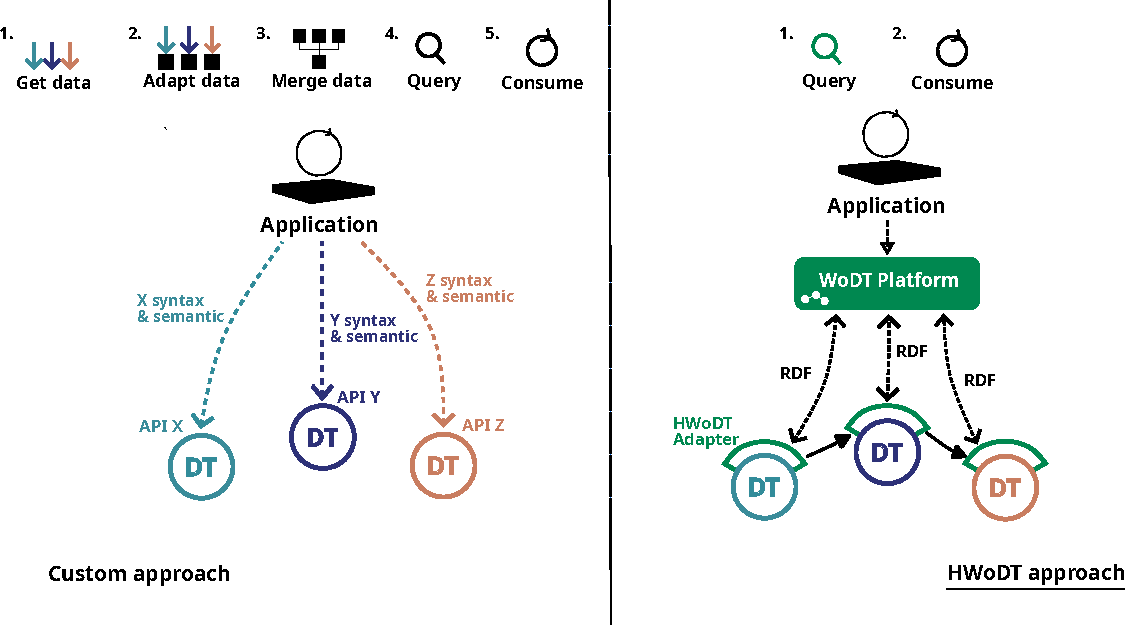
\includegraphics[width=0.75\textwidth]{figures/hwodt/comparison_custom_hwodt.pdf}
  \caption{Comparison of the steps required to perform a ``query'' across heteregenous \acp{DT} versus with the \ac{HWoDT} approach, which abstracts heterogeneity through a uniform interface.}
  \label{fig:comparison-custom-vs-hwodt}
\end{figure*}

A result of the \ac{HWoDT} decoupling is that developers can focus only on application logic, abstracting away the complexity of heterogeneous \ac{DT} integration.  
This yields two important advantages:  
\begin{inlinelist}
    \item the application layer is more stable as it remains unaffected by the introduction of new \acp{DT};
    and  
    \item the \ac{DT} layer can evolve or replace underlying implementations without affecting upper layers as long as the exposed interface is not changed.
\end{inlinelist}

\paragraph{Navigation}
Compatibility with the Linked Data Principles enables consumers to navigate \ac{DT} relationships within the \ac{DTE}, discovering entities and retrieving state information.
%
While this is feasible in homogeneous \acp{DTE} -- such as \azureTwin{} -- where relationships are confined within the same instance, the hypermedia layer of the \ac{HWoDT} addresses this limitation by enabling the definition of cross-platform \ac{DT} relationships using \ac{URI}.   
This enhances the expressiveness of \acp{DTE} and allows developers to model ecosystems that more accurately reflect domain knowledge.
%
As an example, in our trauma management use case, we can link patients with the mission handling their trauma in the \ac{DTE} \ac{KG} despite the respective \acp{DT} being implemented with different technologies as shown in \Cref{lst:mission-dtkg}.
\lstinputlisting[
    caption={A fragment of the \ac{DTE} \ac{KG} showing the representation of the Mission \ac{DT} showing the relationship with the patient.},
    label={lst:mission-dtkg},
]{listings/hwodt/use-case/dtkg-missiondt.ttl}

% \lstinputlisting[
%     caption={Portion of the Ambulance \ac{DTD} that shows the relevant data for the \texttt{SetDestinationCommand} action},
%     label={lst:ambulance-dtd},
% ]{listings/hwodt/use-case/ambulance-dtd.json}    

\paragraph{Explicit Semantics and Interoperability}

The explicit semantic representation in the \ac{HWoDT} is both a tool to support easy integration of different \acp{DT} and a deliberate choice to push the importance of establishing shared semantics so that users can get more information on \ac{DT} functionalities.

Furthermore, the \ac{HWoDT} does not enforce the adoption of a single ontology: while \acp{DT} expose a uniform \ac{DTD}, their \ac{DTKG} content may rely on different vocabularies or ontologies.
This is intentional: to support \acp{DT} from diverse application domains, the framework allows varying ontologies within the same \ac{DTE}.  
Semantic uniformity is thus delegated either to \ac{DT} designers -- who may agree on shared representations -- or to different implementations of the \ac{WoDT} platform, which may translate and align models to a common vocabulary. 
%
In the use case, using the HL7 FHIR standard to unify data from different sources greatly improves the quality of the information in the \ac{DT} ecosystem.

Of course, we acknowledge this requires an additional effort when developing (or mapping) \acp{DT}, as the appropriate domain ontologies need to be identified and used.
Nevertheless, we consider this a valuable trade-off aligned with the efforts towards \ac{DT} interoperability~\cite{Klar_Arvidsson_Angelakis_2024} and the support for defining some level of semantics available in many \ac{DT} tools (including, for instance, \azureTwin{} and Ditto).

% \paragraph{Information Loss}
% With any model conversion there is risk of information loss.
% %
% We acknowledge that, despite the metamodel being general enough for most use cases, a potential limitation of the \ac{HWoDT} is that not all \ac{DT} functionalities may be mapped to Web-based interactions with ease (e.g., data-intensive tasks).

% Ideally, though, the existing applications that leverage specific features of a \ac{DT} will still be able to access them, and new applications built for the ecosystem would benefit from the uniform interface instead.

\paragraph{Performance and Scalability}

As with any additional layer on top of existing systems, performance and infrastructural scalability are a possible concern.
%
In general, the \ac{HWoDT} vision does not target hard real-time scenarios, where dedicated techniques and specialized technologies are required to ensure real-time guarantees.
%
Additionally, even though the preliminary performance measurements show interesting results (\Cref{ssec:performance}), performance optimization was not a primary focus in the development of the \ac{HWoDT} Framework. 
%
Despite this, we can still make some considerations on performances of the whole \ac{HWoDT} approach.

The impact of the translation of a \ac{DT} model to the \ac{DTKG} representation within the adapter is usually negligible, the impact of the adapter depends on its implementation as either an internal (such as in \ac{WLDT}) or external component as in the second case care should be taken to scale the adapter effectively.

The centralized implementation of the platform makes it a potential bottleneck. Specifically -- as confirmed with our preliminary performance tests on the prototype -- interacting with the \ac{DTE} KG is costly because the graph gets updated by all \acp{DT} updates.
%
This is a reasonable trade-off as interacting with the \ac{DTE} provides advanced functionalities that would be impossible or very difficult to replicate simply by interacting with individual \acp{DT}.
%
Nevertheless, we are interested in exploring optimization techniques, as well as decentralized approaches to provide ecosystem services.


\paragraph{Security Considerations}
The openness and Web-based nature of the \ac{HWoDT} approach introduces several security challenges making authentication, authorization, and access control critical.
Although we do not implement this in our prototype yet, standard Web security mechanisms (e.g., OAuth 2.0, HTTPS) can be employed to secure interactions.
Fine-grained access control policies must be enforced both at the data layer (e.g., per-property visibility) and at the hypermedia interface level to possibly restrict access to specific resources.
For instance, \ac{WoT} \ac{TD}-based \ac{DTD} already supports the description of security policies~\cite{wotthing} to define access control of properties and actions. 
Furthermore, provenance tracking and data integrity verification (e.g., using digital signatures) can enhance trust. Namely, \acp{DT} should never be able to modify the representation of another \ac{DT}. Now \ac{DTKG} are not validated, but it should not be possible to post triples updating the description of a different \ac{DT} than the one it is sending them.
Finally, the mapping of a \ac{DT} in its \ac{DTKG} can purposefully avoid exposing sensitive information, or a \ac{DT} could support mechanisms to expose different \acp{DTKG} depending on authorization level of the client.
Existing efforts in the Semantic Web community such as the Solid project\footnote{\url{https://solidproject.org/}} or using RDF-star for access control metadata~\cite{rdfstar-security}, may offer interesting solutions to integrate additional security features on the management of the \ac{DTE} \ac{KG}. 


